\subsection{Technologies in physical layer}

There exist many wireless protocols like IEEE 802.15.4 – ZigBee, IEEE 802.15.1 – Bluetooth, IEEE 802.16 – WiMax or IEEE 802.11a/b/g/n – wireless Lan. Each one of them is suitable for use in different scenario, has different characteristics and may span more than one layer. ZigBee devices are designed for low power consumption, small range and data throughput, which makes them ideal for use in difficult to reach locations where it can run on battery for years. Bluetooth is typically used on devices like smartphones, laptops but also sensors which can run on batter for several days, while being able to achieve higher throughput and short-range communication. On the other hand, 802.11 provides the highest range and throughput but also power consumption, ideal for use in devices being plugged in. Summarising table may be seen in Figure~\ref{fig:protocol-comparison} and more in-depth comparison will follow in later chapter.

\begin{figure}
    \centering
    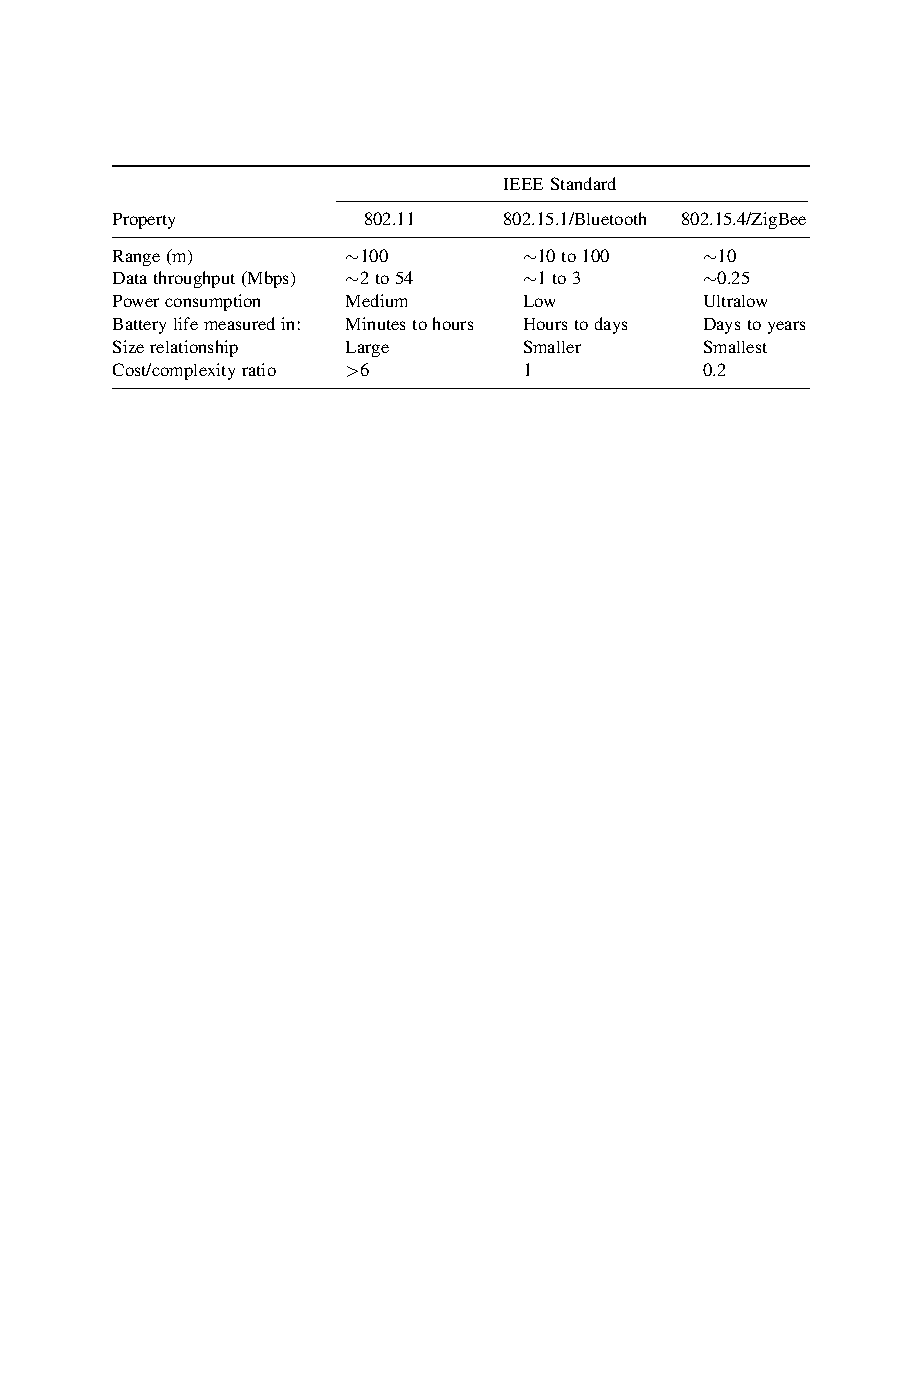
\includegraphics[width=0.8\textwidth]{00images/protocol-comparison}
    \caption{Comparison of IEEE standards for selected physical layer protocols. Taken from~\cite{Sohraby2007WirelessApplications}.}
    \label{fig:protocol-comparison}
\end{figure}